% Enzyme Discovery Agent — project deck
% Build:  pdflatex enzyme_discovery_agent.tex  (run twice)
% Clean, self-contained Beamer theme (no external theme packages required).
\documentclass[aspectratio=169,11pt]{beamer}

\usepackage[T1]{fontenc}
\usepackage[utf8]{inputenc}
\usepackage{helvet}
\renewcommand{\familydefault}{\sfdefault}
\usepackage{graphicx}
\usepackage{tikz}
\usetikzlibrary{arrows.meta,positioning,shapes.geometric}
\usepackage{xcolor}
\graphicspath{{../figures/}}

% ---- palette ----
\definecolor{ink}{HTML}{0F172A}      % near-black slate
\definecolor{muted}{HTML}{475569}    % slate-600
\definecolor{brand}{HTML}{4338CA}    % indigo-700
\definecolor{brand2}{HTML}{0D9488}   % teal-600
\definecolor{accent}{HTML}{E11D48}   % rose-600
\definecolor{soft}{HTML}{EEF2FF}     % indigo-50
\definecolor{rule}{HTML}{CBD5E1}

% ---- clean theme ----
\usecolortheme{default}
\setbeamercolor{normal text}{fg=ink}
\setbeamercolor{frametitle}{fg=brand}
\setbeamercolor{title}{fg=brand}
\setbeamercolor{structure}{fg=brand}
\setbeamercolor{itemize item}{fg=brand2}
\setbeamercolor{itemize subitem}{fg=brand2}
\setbeamerfont{frametitle}{series=\bfseries,size=\LARGE}
\setbeamerfont{title}{series=\bfseries,size=\Huge}
\setbeamertemplate{navigation symbols}{}
\setbeamertemplate{itemize item}{\small\raise0.5pt\hbox{\textbullet}}
\setbeamertemplate{itemize subitem}{\scriptsize\raise0.5pt\hbox{--}}
\setbeamertemplate{frametitle}{%
  \vspace*{0.6em}\hspace*{0.2em}%
  {\usebeamerfont{frametitle}\usebeamercolor[fg]{frametitle}\insertframetitle}\\[-0.2em]
  {\color{rule}\rule{\dimexpr\paperwidth-1.2em\relax}{1.2pt}}\vspace*{-0.2em}}
\setbeamertemplate{footline}{%
  \hbox{}\hfill{\color{muted}\scriptsize Enzyme Discovery Agent\quad\insertframenumber\ /\ \inserttotalframenumber\ }\vspace*{0.5em}}

\newcommand{\hl}[1]{{\color{brand}\textbf{#1}}}
\newcommand{\hlt}[1]{{\color{brand2}\textbf{#1}}}
\newcommand{\hla}[1]{{\color{accent}\textbf{#1}}}
\newcommand{\chip}[2]{\tikz[baseline=(x.base)]{\node[fill=#1!12,draw=#1,rounded corners=3pt,inner sep=3pt,text=#1!75!black,font=\footnotesize\bfseries](x){#2};}}

\title{Enzyme Discovery Agent}
\subtitle{LLM-guided discovery of enzymes for a target reaction}
\author{}
\date{}

\begin{document}

% ---------- Title ----------
{\setbeamertemplate{footline}{}
\begin{frame}[plain]
  \vspace*{1.2em}
  {\color{brand}\rule{\textwidth}{2pt}}\\[1.2em]
  {\Huge\bfseries\color{ink} Enzyme Discovery Agent}\\[0.6em]
  {\LARGE\color{muted} Discovering enzymes for a target reaction —}\\
  {\LARGE\color{muted} without being told the answer}\\[1.4em]
  \chip{brand}{LLM proposes strategy}\quad
  \chip{brand2}{tools + gates find the enzymes}\quad
  \chip{accent}{data-leakage firewall}\\[1.2em]
  {\color{brand}\rule{\textwidth}{2pt}}
\end{frame}}

% ---------- The problem ----------
\begin{frame}{The problem}
  \begin{columns}[T]
    \begin{column}{0.56\textwidth}
      \textbf{Given} a target reaction — substrate(s) $\rightarrow$ product —
      \textbf{find the enzymes} that could catalyze it.\\[0.8em]
      Hard because:
      \begin{itemize}
        \item the reaction is often \hl{novel / non-natural} — no enzyme is annotated for it
        \item the answer must be \hl{discovered}, not looked up
        \item the space is huge: $>$200M UniProt sequences, thousands of folds
      \end{itemize}
      \vspace{0.6em}
      \textbf{The trap:} an agent that is \hla{told the answer family} isn't
      discovering anything.
    \end{column}
    \begin{column}{0.44\textwidth}
      \centering
      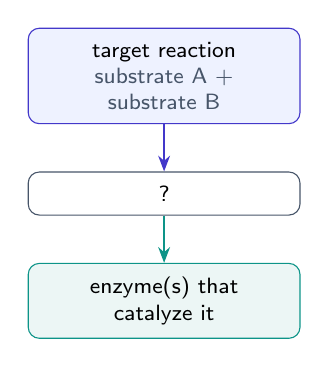
\begin{tikzpicture}[node distance=6mm,every node/.style={font=\footnotesize}]
        \node[draw=brand,rounded corners,fill=soft,text width=3.1cm,align=center,inner sep=5pt] (s) {target reaction\\ \textcolor{muted}{substrate A + substrate B}};
        \node[below=of s,draw=muted,rounded corners,text width=3.1cm,align=center,inner sep=5pt] (q) {?};
        \node[below=of q,draw=brand2,rounded corners,fill=brand2!8,text width=3.1cm,align=center,inner sep=5pt] (e) {enzyme(s) that\\ catalyze it};
        \draw[-{Stealth[length=2mm]},brand,thick] (s)--(q);
        \draw[-{Stealth[length=2mm]},brand2,thick] (q)--(e);
      \end{tikzpicture}
    \end{column}
  \end{columns}
\end{frame}

% ---------- Core principle ----------
\begin{frame}{The core principle}
  \begin{center}
    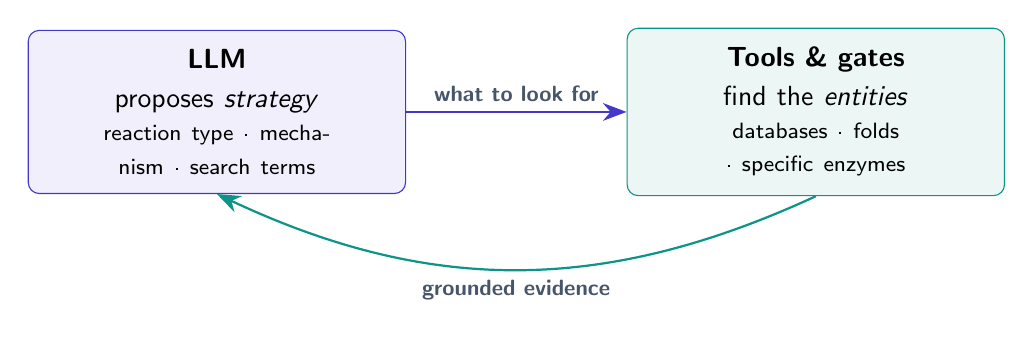
\begin{tikzpicture}[every node/.style={font=\small},node distance=10mm]
      \node[draw=brand,fill=brand!8,rounded corners,text width=4.3cm,align=center,inner sep=7pt,font=\bfseries] (llm)
        {LLM\\[2pt]\normalfont proposes \emph{strategy}\\ \normalfont\footnotesize reaction type · mechanism · search terms};
      \node[right=28mm of llm,draw=brand2,fill=brand2!8,rounded corners,text width=4.3cm,align=center,inner sep=7pt,font=\bfseries] (tools)
        {Tools \& gates\\[2pt]\normalfont find the \emph{entities}\\ \normalfont\footnotesize databases · folds · specific enzymes};
      \draw[-{Stealth[length=3mm]},thick,brand] (llm) -- node[above,font=\footnotesize\bfseries,text=muted]{what to look for} (tools);
      \draw[-{Stealth[length=3mm]},thick,brand2] (tools.south) to[bend left=25] node[below,font=\footnotesize\bfseries,text=muted]{grounded evidence} (llm.south);
    \end{tikzpicture}
  \end{center}
  \vspace{0.4em}
  \begin{columns}[T]
    \begin{column}{0.5\textwidth}
      \hla{Data-leakage firewall} (enforced):
      \begin{itemize}
        \item no answer enzyme / substrate / family in \emph{any} prompt, tool, or comment
        \item ground truth lives \hl{only} in a held-out test oracle the agent never sees
      \end{itemize}
    \end{column}
    \begin{column}{0.5\textwidth}
      \hlt{Grounded \& deterministic}:
      \begin{itemize}
        \item code extracts evidence (direction, substrate fit, correspondence)
        \item no hand-tuned relevance thresholds — relative ranking, not magic numbers
      \end{itemize}
    \end{column}
  \end{columns}
\end{frame}

% ---------- Pipeline overview ----------
\begin{frame}{The pipeline}
  \vspace{0.3em}
  \begin{center}
    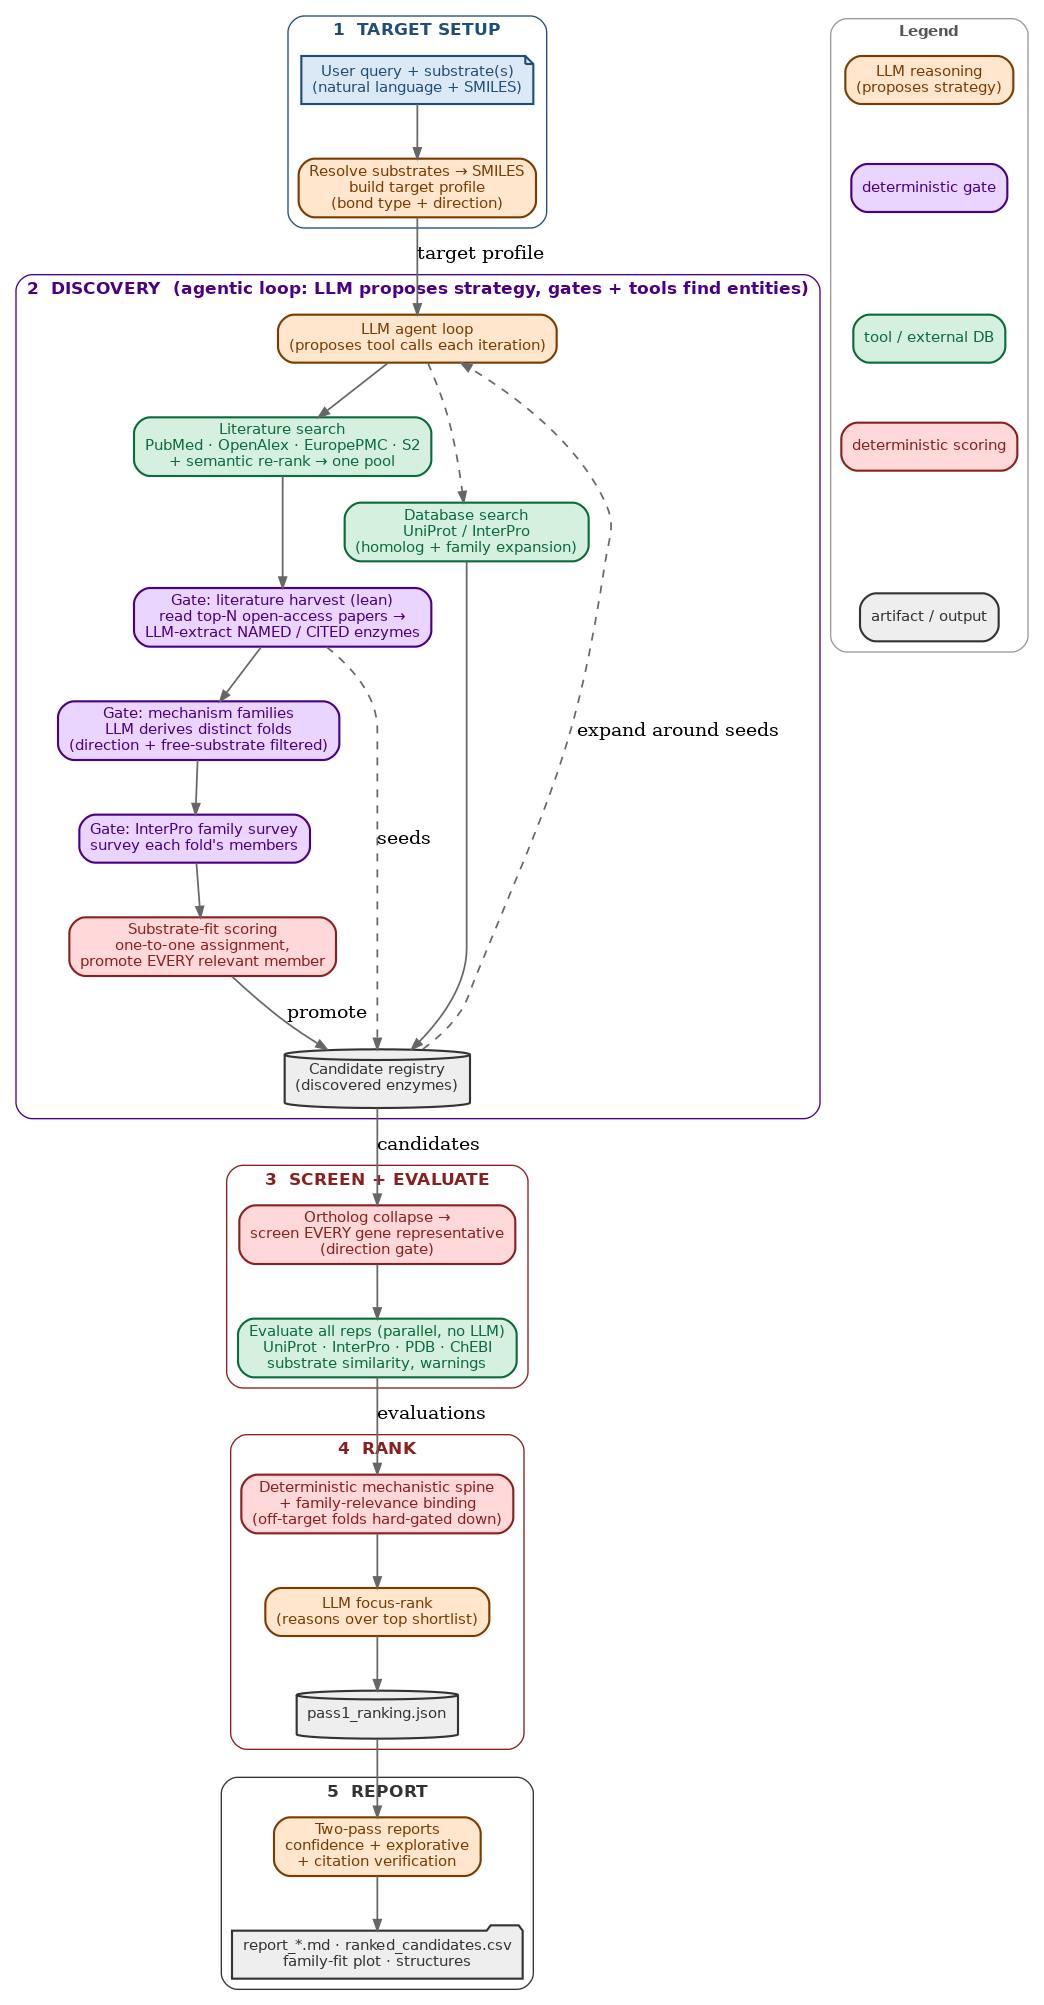
\includegraphics[width=0.99\textwidth]{pipeline_workflow.png}
  \end{center}
  \vspace{0.2em}
  {\footnotesize\color{muted} Five stages. A deterministic \textbf{gate} layer turns optional tools
  into a reliable pipeline; the LLM still drives strategy inside the loop.}
\end{frame}

% ---------- Stage 2 discovery ----------
\begin{frame}{Discovery: three complementary channels}
  \begin{columns}[T]
    \begin{column}{0.33\textwidth}
      \chip{brand}{Literature}\\[0.5em]
      \footnotesize
      Read a few open-access papers; LLM-extract \hl{named / cited} enzymes.
      The \emph{only} route to enzymes named only in a recent paper — reached the
      answer's own biosynthetic cluster.
    \end{column}
    \begin{column}{0.33\textwidth}
      \chip{brand}{Mechanism families}\\[0.5em]
      \footnotesize
      LLM derives the distinct \hl{folds / activation chemistries} for the target
      bond, filtered by \hlt{reaction direction} (a cleavage fold can't serve a
      formation target).
    \end{column}
    \begin{column}{0.33\textwidth}
      \chip{brand}{InterPro survey}\\[0.5em]
      \footnotesize
      Survey each fold's members; score \hl{native-substrate resemblance}; promote
      the good ones to candidates — the primary discovery engine.
    \end{column}
  \end{columns}
  \vspace{1.0em}
  \begin{center}
  \fbox{\parbox{0.92\textwidth}{\centering \small
    \textbf{Design rule:} substrate-awareness lives at the \hl{member} level, not the
    family archetype — a fold's textbook substrate $\neq$ its member range.}}
  \end{center}
\end{frame}

% ---------- One-to-one ----------
\begin{frame}{Judging substrate fit: one-to-one assignment}
  \begin{columns}[T]
    \begin{column}{0.5\textwidth}
      A two-substrate target must not \hla{flatter itself}: without one-to-one
      assignment, \emph{both} target substrates match the enzyme's single best
      native, hiding a poor second partner.\\[0.6em]
      \hlt{Fix (shared by promotion \& ranking):} each native serves \hl{at most one}
      target substrate; the score is the \emph{worst} assigned pair (the bottleneck).\\[0.6em]
      {\footnotesize\color{muted} So a target amine is forced onto the family's amine
      partner — even a tiny functional-group-less donor scores as the poor fit it is.}
    \end{column}
    \begin{column}{0.5\textwidth}
      \centering
      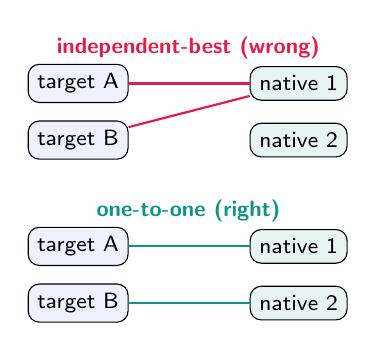
\begin{tikzpicture}[every node/.style={font=\footnotesize},yscale=0.9]
        \node[text=accent,font=\footnotesize\bfseries] at (1.4,2.5) {independent-best (wrong)};
        \node[draw,rounded corners,fill=soft] (t1) at (0,2) {target A};
        \node[draw,rounded corners,fill=soft] (t2) at (0,1.2) {target B};
        \node[draw,rounded corners,fill=brand2!10] (n1) at (2.8,2) {native 1};
        \node[draw,rounded corners,fill=brand2!10] (n2) at (2.8,1.2) {native 2};
        \draw[accent,thick] (t1)--(n1);
        \draw[accent,thick] (t2)--(n1);
        \node[text=brand2,font=\footnotesize\bfseries] at (1.4,0.2) {one-to-one (right)};
        \node[draw,rounded corners,fill=soft] (u1) at (0,-0.3) {target A};
        \node[draw,rounded corners,fill=soft] (u2) at (0,-1.1) {target B};
        \node[draw,rounded corners,fill=brand2!10] (m1) at (2.8,-0.3) {native 1};
        \node[draw,rounded corners,fill=brand2!10] (m2) at (2.8,-1.1) {native 2};
        \draw[brand2,thick] (u1)--(m1);
        \draw[brand2,thick] (u2)--(m2);
      \end{tikzpicture}
    \end{column}
  \end{columns}
\end{frame}

% ---------- Don't drop ----------
\begin{frame}{Discovery means: don't drop relevant enzymes}
  \begin{columns}[T]
    \begin{column}{0.5\textwidth}
      \hl{Promote every relevant member}\\
      {\footnotesize The survey no longer keeps only a fold's top-2 by fit — every
      same-direction, substrate-resolved member becomes a candidate. A 24-member
      fold's long tail is kept, not thrown away.}\\[1.0em]
      \hl{Evaluate every representative}\\
      {\footnotesize Evaluation is deterministic (network only, no LLM), so breadth
      is free. Every distinct gene is evaluated in parallel — no eval-budget cap
      silently drops a relevant enzyme.}
    \end{column}
    \begin{column}{0.5\textwidth}
      \centering
      \vspace{0.5em}
      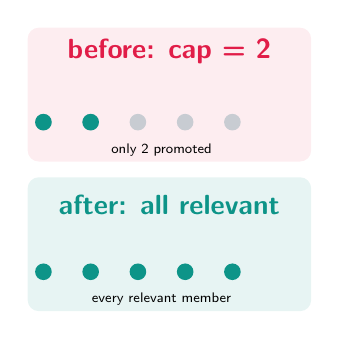
\begin{tikzpicture}[font=\footnotesize]
        \fill[accent!8,rounded corners] (-0.2,-0.2) rectangle (3.4,1.5);
        \node[text=accent,font=\bfseries] at (1.6,1.2) {before: cap = 2};
        \foreach \i in {0,...,4}{\fill[muted!30] (\i*0.6,0.3) circle (3pt);}
        \fill[brand2] (0,0.3) circle (3pt); \fill[brand2] (0.6,0.3) circle (3pt);
        \node at (1.5,-0.05) {\tiny only 2 promoted};
        \fill[brand2!10,rounded corners] (-0.2,-2.1) rectangle (3.4,-0.4);
        \node[text=brand2,font=\bfseries] at (1.6,-0.75) {after: all relevant};
        \foreach \i in {0,...,4}{\fill[brand2] (\i*0.6,-1.6) circle (3pt);}
        \node at (1.5,-1.95) {\tiny every relevant member};
      \end{tikzpicture}
      \\[0.4em]
      {\footnotesize\color{muted} Cost rises; discovery quality is the priority.}
    \end{column}
  \end{columns}
\end{frame}

% ---------- Ranking ----------
\begin{frame}{Ranking: grounded first, LLM second}
  \begin{itemize}
    \item \hl{Deterministic mechanistic spine} orders by grounded evidence
      (bond change, direction, substrate fit) — reproducible, no magic weights.
    \item \hlt{Family-relevance binding}: members of a fold the agent \emph{stopped}
      (off-target chemistry) are hard-gated to the bottom; on-target folds float up.
    \item \hl{LLM focus-rank} reasons over only the top shortlist — a thin,
      auditable layer on top of the deterministic order.
  \end{itemize}
  \vspace{0.6em}
  \begin{center}
    \tikz[baseline]{\node[draw=brand,rounded corners,fill=brand!6,inner sep=6pt,font=\footnotesize]{%
      direction hard-gate\ \ $\rightarrow$\ \ substrate-fit bottleneck\ \ $\rightarrow$\ \ family binding\ \ $\rightarrow$\ \ LLM focus-rank};}
  \end{center}
\end{frame}

% ---------- Results ----------
\begin{frame}{Validation}
  \small
  Benchmark (ground truth in the held-out oracle only): find amide synthetases that
  ligate a C\textsubscript{6} diacid + a C\textsubscript{6} diamine — enzymatic
  nylon-6,6 precursors.
  \vspace{0.4em}
  \begin{columns}[T]
    \begin{column}{0.52\textwidth}
      \textbf{What the run recovers}
      \begin{itemize}\small
        \item top ranks: NIS / ANL amide synthetases — genuine \hl{substrate analogues}
          (citrate–diamine ligases)
        \item \hlt{DdaG} (the strict answer) recovered at \#4 — via the \hl{literature}
          channel, in the answer's own gene cluster
        \item family list \hl{direction-clean} (no cleavage folds); CARNS1-type
          over-ranking gone
      \end{itemize}
    \end{column}
    \begin{column}{0.48\textwidth}
      \textbf{Cost / behavior}
      \begin{itemize}\small
        \item wall-clock \hlt{53\,min $\rightarrow$ 32\,min} after the lean-literature change
        \item run is \hla{98\% LLM-inference} bound; tools are $\sim$2\%
        \item every screened candidate evaluated (no budget drop)
      \end{itemize}
      \vspace{0.4em}
      {\footnotesize\color{muted} Ground truth is used only to score \emph{after} the
      run — never fed to the agent.}
    \end{column}
  \end{columns}
\end{frame}

% ---------- This work ----------
\begin{frame}{Recent work: correctness + efficiency + cleanup}
  \begin{columns}[T]
    \begin{column}{0.5\textwidth}
      \hlt{Discovery quality}
      \begin{itemize}\small
        \item one-to-one substrate assignment (shared by promotion \& ranking)
        \item promote \emph{every} relevant member; evaluate \emph{every} representative
        \item direction-clean mechanism families
      \end{itemize}
      \vspace{0.5em}
      \hl{Efficiency}
      \begin{itemize}\small
        \item lean literature harvest: $\sim$90\% fewer harvest LLM calls, no open-access wall
        \item parallel evaluation
      \end{itemize}
    \end{column}
    \begin{column}{0.5\textwidth}
      \hla{Refactor} (behavior-preserving)
      \begin{itemize}\small
        \item unified 9 gates into one pipeline ritual
        \item de-duplicated scoring / direction logic
        \item $\sim$730 lines of dead code removed
      \end{itemize}
      \vspace{0.5em}
      \begin{center}
        \chip{brand2}{215 tests green}\quad\chip{brand}{firewall-clean}
      \end{center}
    \end{column}
  \end{columns}
\end{frame}

% ---------- Limitations ----------
\begin{frame}{Limitations \& next steps}
  \begin{itemize}
    \item \hl{Literature recall} — the field's best papers are missed on search
      \emph{vocabulary} (and paywalls); query reformulation helps but is stochastic.
    \item \hl{Speed} — the loop is LLM-inference bound (60k-token prompts); levers are
      prompt pruning + parallel / fewer finalization passes.
    \item \hl{Ranking quality} — unify the remaining scoring formulas; validate the
      one-to-one change end-to-end on the benchmark.
    \item \hl{Coverage} — make family-member enumeration substrate-aware and complete.
  \end{itemize}
  \vspace{0.8em}
  \begin{center}\small\color{muted}
    Every change: suite-green, firewall-clean, documented in an append-only devlog.
  \end{center}
\end{frame}

% ---------- Closing ----------
{\setbeamertemplate{footline}{}
\begin{frame}[plain]
  \vspace*{2.0em}
  {\color{brand}\rule{\textwidth}{2pt}}\\[1.0em]
  {\LARGE\bfseries\color{ink} Discover, don't look up.}\\[0.8em]
  {\large\color{muted} LLM proposes the strategy · grounded gates and tools find the enzymes ·}\\
  {\large\color{muted} a firewall keeps the answer out of the agent.}\\[1.4em]
  \chip{brand}{one-to-one substrate fit}\quad
  \chip{brand2}{promote \& evaluate everything relevant}\quad
  \chip{accent}{no answer leakage}\\[1.0em]
  {\color{brand}\rule{\textwidth}{2pt}}
\end{frame}}

\end{document}
